
\chapter{Literatuurstudie}

\section{Dienstregeling openbaar vervoer}

Interoperabiliteit van datasets is belangrijk om routeplanning over verschillende vervoersmaatschappijen toe te laten. Als je jouw reis wil verderzetten van een bus naar een trein zul je hoogstwaarschijnlijk een ander transportbedrijf gebruiken. De tijdstabellen moeten als het ware dezelfde "taal" spreken om die samen te laten werken. 

\subsection{GTFS}
In 2005 introduceerde Google een specificatie om transportdata uniformiteit te verzekeren, genaamd General Transit Feed Specification (GTFS) \cite{gtfs-ref}. GTFS is een set van regels die om statische tijdstabellen in op te stellen. Deze specificeert welke bestanden noodzakelijk en optioneel zijn en welke informatie hierin verplicht en optioneel is. Deze bestanden zijn opgesteld volgens het Comma Seperated Values (CSV) formaat.
Niet alle bestanden zijn noodzakelijk voor deze masterproef. Zie \cite{gtfs-ref} voor de volledige documentatie. Hieronder volgt een uitleg van de meest gebruikte termen en bestanden.

\subsubsection{Terminologie}

Een \textit{stop} is een plaats waar een voertuig stopt, dit kan gaan om een perron, bushalte etc. Elke ov-bedrijf bestaat uit een aantal \textit{routes}. Dit zijn vastgelegde trajecten, bijvoorbeeld het traject tussen Gent Flanders Expo - Wondelgem waartussen tram 1 van De Lijn rijdt. \textit{Trips} zijn de effectieve trajecten die afgelegd worden door een voertuig. Zo zijn er meestal meerdere trips die eenzelfde route afleggen. Tram 1 legt meerdere keren per dag eenzelfde route af. Er zijn ook meerdere trips voor een route, omdat niet elke trip op dezelfde plaatsen stopt. Het kan gerust gebeuren dat er een stopplaats wordt overgeslagen. Deze trips worden gegroepeerd per dag en worden voorgesteld door een \textit{service}. Wil je weten welke routes op een bepaalde dag X rijden, dan moet je ophalen welke services die dag rijden. Dan kun je terugvinden welke routes deze representeren. Een andere belangrijke term is \textit{stoptime}. Dit houdt in wanneer een voertuig tijdens een trip op een bepaalde stopplaats aankomt en terug vertrekt.

Zoals je kan opmerken is routeplanning een verwarrend woord in de context van GTFS. Dit kan gezien worden als het combineren van verschillende trips.

\subsubsection{Gebruikte bestanden}

Volgens GTFS zijn er zes bestanden verplicht en zeven bestanden optioneel. Deze masterproef doelt enkel op het verbeteren van de basisfunctionaliteit van routeplanning waardoor data over tarieven, spoorvormen etc. niet nodig zijn.

Van elke GTFS \textit{feed} worden er vijf bestanden gebruikt:
\begin{itemize}
	\item trips.txt. Dit bestand zorgt voor de mapping tussen trip, een route en service.
	\item routes.txt. Bevat een overzicht van alle routes.
	\item calendar\_dates.txt. Dit bestand bevat voor elke dag welke services er rijden. Normaal wordt een calendar.txt bestand gebruikt om services te mappen op de dagen dat ze rijden en wordt calendar\_dates.txt enkel gebruikt voor uitzonderingsdagen. In de realiteit gebruiken de meeste ov-bedrijven enkel dit bestand om de dagen op te lijsten. Daarom werd er voor gekozen om enkel hierop toe te spitsen.
    	\item stoptimes.txt.Dit bestand bestaat uit een verzameling stopplaatsen met telkens de aankomst- en vertrektijden bij.
	\item stops.txt bevat een lijst met informatie over alle stopplaatsen. Dit speelt een belangrijke rol om interoperabiliteit tussen verschillende datasets te voorzien. Later hierover meer (hoofdstuk \ref{resultaten}).
\end{itemize}

Deze bestanden bevatten enkel gegevens voor statische tijdstabellen. Om realtime informatie mogelijk te maken is een extra laag bovenop GTFS gemaakt, genaamd GTFS-RT.

\subsection{GTFS-RT}

General Transit Feed Specification RealTime (GTFS-RT) bevat actuele informatie over bepaalde trips, routes, stops... van de corresponderende GTFS feed. Dit kan gaan van vertragingen en onvoorziene omstandigheden tot de exacte huidige positie van een voertuig. Deze data wordt met Protocol buffers, een binair formaat, geserialiseerd om zo compact mogelijk te zijn. Uiteindelijk worden de GTFS-RT bestanden ter beschikking gesteld via een webserver.

Nu we hebben gezien hoe transportdata wordt vrijgegeven, kunnen we afvragen hoe verschillende datasets gecombineerd kunnen worden. Een van de methodes om dit op te lossen is er voor te zorgen dat machines begrijpen waarover deze data gaat. GTFS data kan gebruikt worden in programma's, maar enkel een mens begrijpt wat er bedoeld wordt met bepaalde headers. In volgende sectie bekijken we welke mogelijkheden het semantische web hiervoor biedt.

\section{Semantisch web}

Het semantisch web is een verzameling technologi\"een (URI, RDF, SPARQL, ontologi\"en...) die het mogelijk maakt om informatie op het web machine-leesbaar te maken. Concepten, termen en relaties binnen een bepaald domein worden met elkaar gelinkt waardoor het mogelijk is om informatie te achterhalen dat aanvankelijk niet aanwezig was. Sommige technologi\"en zoals SPARQL worden niet gebruikt voor de uiteindelijke implementatie van deze masterproef, maar als middel om analogie te vinden met de huidige problemen van routeplannen. 

\subsection{RDF}

Resource Description Framework (RDF)\cite{RDF11-CONCEPTS} is een conceptueel model om bronnen op het web weer te geven. Een feit wordt als atomaire eenheid beschouwd om kennis weer te geven. Zo is het mogelijk om nieuwe feiten te destilleren als verschillende feiten over dezelfde zaken gaan. Dit is een andere manier om objecten weer te geven dan de typische object geori\"enteerde omgeving van klassen en attributen.
Een feit \footnote{Deze drieledige structuur wordt ook \textit{triple} of \textit{tuple} genoemd. } bestaat uit drie elementen: subject, predikaat en object. Dit kan je als een zin lezen met een onderwerp, werkwoord en lijdend voorwerp, bijvoorbeeld "route 123 heeft als aanduiding `Brussel - Gent'". Hierbij is 'route 123' het onderwerp, 'aanduiding' de relatie en 'Brussel - Gent' de waarde van het onderwerp. Het object kan een vaste waarde of een ander object zijn.

\begin{figure}[h!]
\centering
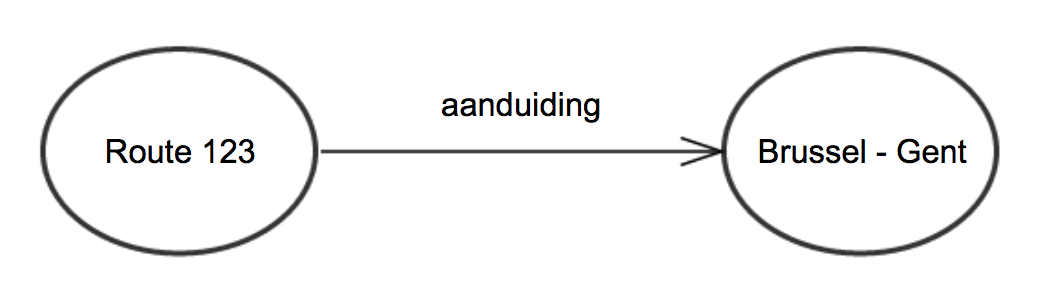
\includegraphics[width=0.5\textwidth]{rdf.png}
\caption{RDF representatie van een triple}
\end{figure}

Een RDF model is dus een gerichte graaf waarbij de knopen en verbindingen benoemd zijn. Er ontstaat als het ware een web van verschillende concepten die met elkaar verweven worden. Data die op zo'n manier opgebouwd is, wordt \textit{Linked Data} genoemd. Om in de praktijk te kunnen refereren naar bepaalde bronnen, zal er identificatie van concepten nodig zijn.

\subsection{Bronidentificatie}
\label{subsec:uri}
Met RDF hebben we een model om bronnen met elkaar te linken en zo feiten te cre\"eren. Om geen verwarring tussen verschillende bronnen te hebben, wordt er gebruik gemaakt van HTTP Universal Resource Identifiers (URI) op het web. Dit heeft dezelfde structuur als een Universal Resource Locator (URL) die in de adresbalk van een browser ingegeven wordt. URI's worden gebruikt om te identificeren, terwijl URL's gebruikt worden om documenten te localiseren. Het kan dus zijn dat een URI een URL is als deze naast identificeren ook gebruikt wordt om meer informatie over te vinden. Het opzoeken van meer informatie over een bepaald onderwerp noemt men \textit{derefereren}.
Neem nu een boek met als IBCN nummer 123 uit een bibliotheek, deze kan ge\"identificeerd worden via \textit{https://bibliotheek.org/books/123}. Als andere bronnen, zoals de auteur, informatie bevatten over dit boek, dan kan er zonder verwarring verwezen worden hiernaar.

Net zoals je bij object geori�nteerd programmeren worden er klasses met bepaalde attributen gemaakt om concepten uit de echte wereld zo re\"eel mogelijk weer te geven. In de wereld van het semantisch web wordt hiervoor gebruik gemaakt van vocabularia.

\subsection{Vocabularium}
Een vocabularium/ontologie is een verzameling klasses en eigenschappen die binnen een bepaalde context samenhoren. Zo is RDF zelf ook een vocabularium waarbij bronnen ofwel een subject, predikaat of object voorstellen. Op dit niveau horen alle bronnen simpelweg tot dezelfde context van triples. Om zaken uit de echte wereld samen te steken, zijn er twee vocabularia die daarbij kunnen helpen: Resource Description Framework Schema (RDFS) en Web Ontology Language (OWL). Met deze vocabularia worden er extra elementen ge�ntroduceerd waarmee er gespecificeerd kan worden of een bron een klasse, eigenschap, waarde of datatype voorstelt. 

Zo werd er voor GTFS data ook een vocabularium\footnote{vocab.gtfs.org/terms} opgesteld. Als we dit toepassen op het voorbeeld van daarnet, zien we dat een triple wordt voorgesteld door 2 URI's en een waarde voor het object.

\begin{figure}[h!]
\centering
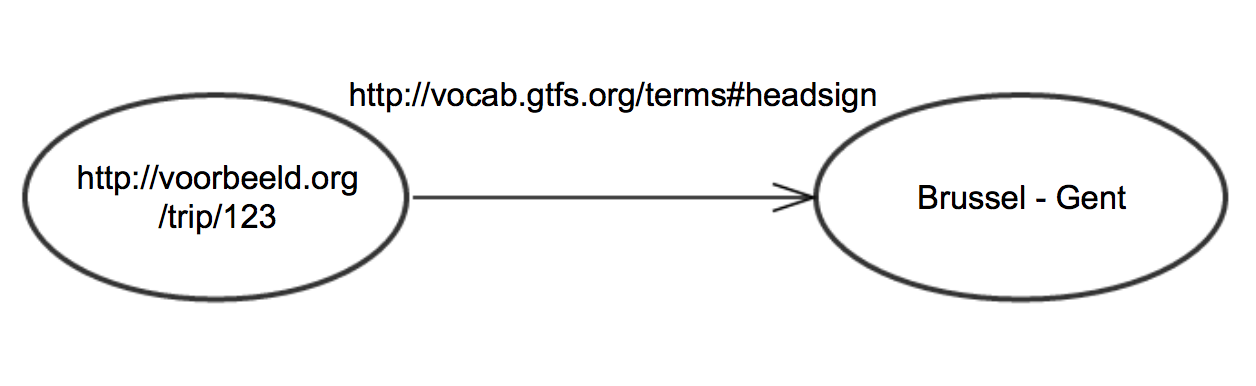
\includegraphics[width=0.5\textwidth]{rdfvocab.png}
\caption{Triple met URI's}
\end{figure}

Om een toepassing te kunnen bouwen wordt data in een bepaald formaat gegoten. Extensible Markup Language (XML) en JavaScript Object Notation (JSON) zijn meest bekende voor webapplicaties te bouwen. Voor beiden is er een uitbreiding voor Linked Data gemaakt: RDF/XML en JSON-LD. Doordat JSON als standaard dataformaat op het web beschouwd wordt zullen we enkel dieper ingaan op JSON-LD.

%\subsection{Re\"ificatie}
%
%%Om niet telkens de volledige URI te moeten typen wordt er gebruik gemaakt van prefixen. Volgende prefix wordt gebruikt in de voorbeelden:
%%PREFIX vb: <http://voorbeeld\#>
%
%Nu dat we een collectie triples hebben, willen we meer informatie over bepaalde triples zelf. (Is het mogelijk om alle triples met bepaald subject of subject+predikaat te re\"ificeren?) Om dit te kunnen doen wordt de triple in zijn geheel als bron behandeld. Dit proces wordt re�ficatie genoemd.
%Stel, we hebben volgende triple: subject: ?ex:trein123?, predikaat: ?ex:isGestationeerdIn?, object: ?ex:Rijsel?. Voor een transportbedrijf kan het handig zijn om te weten welke conducteur de trein heeft gestationeerd. Om deze informatie toe te voegen aan de triple, wordt er een subject gemaakt met als type rdf:statement:
%
%\begin{lstlisting}[label=reificatie,caption=Re\"ificatie van een triple]
%ex:treinStationering1            rdf:type    rdf:statement
%ex:treinStationering1            rdf:subject    ex:trein123
%ex:treinStationering1            rdf:predicate    ex:isGestationeerdIn
%ex:treinStationering1            rdf:object    stations:Rijsel
%ex:treinStationering1        rdf:conducteur    conducteurs:1
%\end{lstlisting}
%
%Nu hebben we een attribuut toegevoegd over onze oorspronkelijke triple. Wat we willen is een context toevoegen aan een collectie triples. Een context wordt net als een andere bron ge�dentificeerd met een URI. Deze wordt simpelweg als attribuut toegevoegd aan de triples.
%
%Dit zorgt uiteraard voor onnodig veel extra triples:
%
%TO = aantal originele triples
%TN = aantal nieuwe triples
%$\rightarrow$ TN = 3 x TO + 1
%

\subsection{JSON-LD}

Als je de openingsuren van een winkel opzoekt in een zoekmachine, gebeurt het vaak dat je een overzicht met informatie bekomt zonder te moeten verderklikken naar een website. Meestal wordt er gebruik gemaakt van JSON-LD om deze informatie aan zoekmachines duidelijk te maken.
JSON-LinkedData is dus een serialisatie formaat voor gelinkte data. Het grote voordeel van JSON-LD is de compabiliteit met bestaande tools die met JSON werken. Zo kan een JSON-LD document als apart script bestand toegevoegd worden aan een website om semantische informatie weer te geven. 
Een JSON-LD document bestaat uit twee delen: een context die bepaalt hoe de data ge\"interpreteerd moet worden en de data zelf. Listing\ref{routejson} bevat informatie over het route voorbeeld in JSON.

\begin{lstlisting}[label=routejson,caption=Voorbeeld trip in JSON.]
{
	"trip id": "trip 123",
	"aanduiding": "Brussel - Gent"
}
\end{lstlisting}

Om deze informatie semantisch te beschrijven, wordt er context toegevoegd. In listing \ref{tripjsonld}  gebruiken we als context de Linked GTFS ontologie. Het type 'trip' wordt toegevoegd met het sleutelwoord '@type'. Er is ook een \textit{prefix} 'trip:' toegevoegd om de leesbaarheid te verhogen. Het is een goede gewoonte om elke bron een eigen identificering geven met behulp van '@id'.

\begin{lstlisting}[label=tripjsonld,caption=Voorbeeld trip in JSON-LD.]
{
	"@context": "http://vocab.gtfs.org/terms",
	"@type": "Trip",
	"trip": "http://voorbeeld.org/trips/",
	"@id": "trip:123",
	"shortName": "trip 123",
	"headsign": "Brussel - Gent"
}
\end{lstlisting}

Dit JSON(-LD) object bevat nu enkel informatie over de entiteit 'trip:123'. Als er meerdere trips zijn met dezelfde context is het handiger om gebruik te maken van benoemde grafen (Engels: \textit{Named Graphs}).

\subsection{Benoemde grafen}

Triples kunnen onderverdeeld worden in grafen. Dit is handig om eigenschappen, metadata... toe te kennen aan een groep triples. In hoofdstuk \ref{subsec:hypermedia} zal blijken dat dit voor hypermedia API's een belangrijke rol speelt. De oorspronkelijke triple is nu een quad geworden met \textit{\textless graaf\textgreater \textless subject\textgreater \textless predikaat \textgreater \textless object\textgreater}. Een voorwaarde is dat de graaf zelf ook ge\"identificeerd wordt met een URI zodat er van buitenaf hiernaar gerefereerd kan worden.

In JSON-LD wordt er gebruik gemaakt van het sleutelwoord '@graph' waarin een array van alle entiteiten van een graaf komt. Listing \ref{tripjsonldgraph} toont hoe makkelijk het is om metadata toe te voegen aan de graaf.

\begin{lstlisting}[label=tripjsonldgraph,caption=Voorbeeld trip in JSON-LD met benoemde graaf.]
{
	"@context": "http://vocab.gtfs.org/terms",
	"dc": "http://purl.org/dc/terms/",
	"dc:publisher": "Brecht Van de Vyvere",
	"@id": "http://voorbeeld.org/graaf/1",
	"@graph":
	[
		{
			"@id": "trip:123",
			"@type": "Trip",
			"trip": "http://voorbeeld.org/trips/",
			"shortName": "trip 123",
			"headsign": "Brussel - Gent"
		}, ...
	]
}
\end{lstlisting}

JSON-LD data kan omgezet worden naar triples om die dan vervolgens in te laden in een triplestore. Hierop kunnen dan vragen afgevuurd worden om informatie te bekomen.

\subsection{SPARQL}
\label{sparql}
SPARQL Protocol and RDF Query Language (SPARQL) is een zoektaal specifiek voor data in RDF formaat. Hiermee kan gelijk welke vraag gesteld worden aan een \textit{triplestore}. In lijst \ref{vbsparqlquery} zie je een voorbeeld SPARQL-query die de URI's van alle verschillende luchthavens in Itali\"e opvraagt.

\begin{lstlisting}[label=vbsparqlquery,caption=Voorbeeld van een SPARQL query.,firstnumber=1]
"SELECT DISTINCT ?entity 
WHERE {
	?entity a dbpedia-owl:Airport;
			dbpprop:cityServed dbpedia:Italy.
}"
\end{lstlisting}

Dit is nu nog een relatief simpele vraag voor een SPARQL-\textit{endpoint}. Het grote probleem \cite{verborgh_ldow_2014} van deze endpoints is dat slechts 30\% effectief 99\% online blijft in een maand. Er is namelijk geen restrictie op het soort queries die uitgevoerd kunnen worden. Voor re\"eele toepassingen is dit ontoelaatbaar dat wanneer veel cli\"ents complexe queries afvuren, de server kan uitvallen.

We zullen eerst het spectrum van \textit{Linked Data fragments} (LDF's) bespreken. Daarna bekijken we een oplossing om SPARQL-endpoints schaalbaar te kunnen query'en.

\subsection{Linked Data Fragments}
\label{ldf}
Een Linked Data dataset is een collectie triples die door een iemand wordt vrijgegeven. Meestal zijn we enkel ge\"interesseerd in bepaalde delen van deze collectie, bijvoorbeeld met een SPARQL-query beschik je enkel over de data die hieraan voldoet. Door een URL te derefereren beschik je enkel over informatie die over dit onderwerp gaat. Deze verschillende interfaces hebben gemeen dat ze een bepaald fragment over eenzelfde dataset voorstellen. In figuur \ref{ldf-as-1} zie je de LDF's as.

\begin{figure}[h!]
\centering
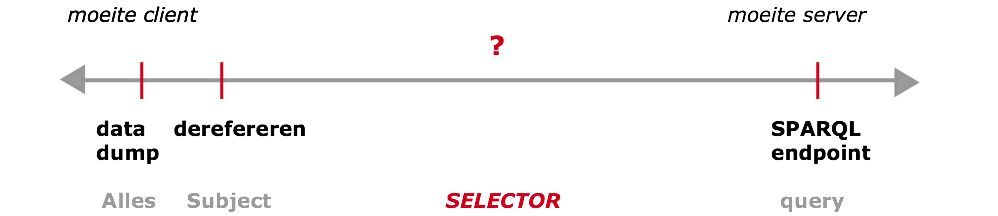
\includegraphics[width=0.8\textwidth]{LDF-as1.png}
\caption{Linked Data Fragments-as}
\label{ldf-as-1}
\end{figure}

Bij elk soort LDF hoort een bepaalde \textit{selector}. Dit is een booleaanse functie die bepaalt of een triple tot het gewenste deel van de dataset behoort of niet. Voor een datadump is deze functie altijd TRUE voor gelijk welke triple. Triples die horen bij een SPARQL-query hebben de query als selector.

Naast data, volgens een bepaalde selector, zijn er nog twee andere eigenschappen die LDF van elkaar onderscheiden:
\begin{itemize}
\item Hypermedia controls. Dit zijn URL's die meer informatie bevatten over bepaalde entiteiten in het fragment, maw informatie over gerelateerde Linked Data Fragmenten. Voor datadumps en het resultaat van een SPARQL query komt dit neer op het derefereren van de URL die een bepaald object voorstelt.
\item Metadata. Dit is informatie over de data zelf, bijvoorbeeld het aantal triples of datum van aanmaak/query'en. Deze informatie wordt in triples toegevoegd aan het datafragment.
\end{itemize}

Het interessante aan deze as is dat verschillende interfaces met elkaar vergeleken kunnen worden. LDF's is dus geen technologie, maar een visie hoe de balans tussen cli\"ent en server kan afgewogen worden. Met data, controls en metadata in het achterhoofd werd in 2014 een oplossing bedacht om Linked Data query'en schaalbaar te maken op het web \ref{tpf}.

\subsection{Triple Pattern Fragments}
\label{tpf}
Bij SPARQL-endpoints (\ref{sparql}) is er een probleem dat endpoints niet 100\% online blijven doordat er geen beperking is in de grootte en complexiteit van queries. Een Triple Pattern Fragments (TPF) is een nieuwe Linked Data Fragment's visie die de trade-off tussen cli\"ent en server afweegt (\ref{ldf-as1b}) door een gulden middenweg te vinden.

\begin{figure}[h!]
\centering
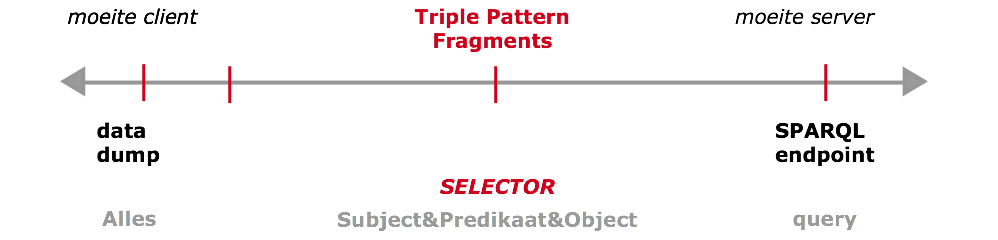
\includegraphics[width=0.8\textwidth]{LDF-as1b.png}
\caption{Linked Data Fragments-as met Triple Pattern Fragments.}
\label{ldf-as1b}
\end{figure}

Deze gulden middenweg houdt twee zaken in:
\begin{itemize}
\item servers bieden een simpele, \textit{low-cost} interface aan.
\item cli\"ents zijn verantwoordelijk voor het oplossen van bepaalde queries. 
\end{itemize}

\subsubsection{Server}
De server is verantwoordelijk voor het teruggeven van triples die voldoen aan een bepaald triple patroon. Zo'n patroon is de combinatie van een subject, predikaat en object waarvan minstens een element een waarde heeft. Een voorbeeld van HTTP template van een TPF-server is te zien in lijst \ref{tpf-interface}. Dankzij hypermedia controls is het mogelijk om een LDF gepagineerd terug te geven. Dit wordt gedaan met behulp van de Hydra hypermedia vocabularium\footnote{http://www.w3.org/ns/hydra/core\#}: hydra:totalItems, hydra:itemsPerPage, hydra:firstPage, hydra : nextPage. Bij \ref{tpf-client} zal het totaal aantal items z'n nut bewijzen.

\begin{lstlisting}[label=tpf-interface,caption=Triple Pattern Fragments interface]
http://triplepatternfragments.org?subject={...}&predikaat={...}&object={...}
\end{lstlisting}

Het berekenen van triples die aan zo'n patroon voldoen is relatief simpel voor een server. Dankzij het beperkt aantal parameters kan er aan HTTP caching gedaan worden. Hierdoor is het mogelijk om veel cli\"ents tegelijk aan te kunnen en is het probleem van SPARQL-endpoints aan de kant geschoven.

\subsubsection{Client}
\label{tpf-client}
Bij SPARQL kon de client gelijk welke vraag stellen aan de server en kreeg daar (hopelijk) antwoord op. Nu is de client verantwoordelijk voor het oplossen van een query door de meerdere simpele vragen te stellen aan de server. Dit gaat ten koste van bandbreedte.

Om het algoritme uit te leggen, gebruiken we het voorbeeld met Italiaanse luchthavens van \ref{vbsparqlquery}. De WHERE-clausule bestaat uit triple patronen: de eerste stelt LDF voor van alle luchthavens en het tweede patroon stelt alle entiteiten die ten dienste van Itali\"e staan. De eerste stap van het algoritme haalt voor beide patronen het eerste fragment op. Dankzij metadata weet de cli\"ent welk patroon het minste triples bevat. Over het resultaat van dit patroon wordt er ge\"iterereerd en worden de variabelen hiervan ingevuld bij de andere WHERE-clausules. Nu wordt hetzelfde algoritme recursief uitgevoerd op de ingevulde, overgebleven WHERE-clausules. Als er in het voorbeeld 1000 luchthavens zijn (eerste patroon), maar slechts 10 entiteiten zijn die Itali\"e dienen (tweede patroon) dan wordt het tweede patroon als startpatroon gekozen. Vervolgens wordt elke triple van dit patroon \textit{gejoint} met het tweede patroon. Als de \textit{count} metadata van deze join een is, weten we dat dit een goed antwoord is.

Zoals je kan zien is TPF een \textit{greedy} algoritme doordat telkens het kleinste LDF van een bepaald patroon gekozen wordt. Een van de voordelen van deze manier van werken is dat het resultaat \textit{gestreamt} kan worden. In tegenstelling tot SPARQL hoeft de cli\"ent niet te wachten op het volledige resultaat om resultaten te tonen aan de gebruiker.

\subsection{Analogie met routeplanning}
Een SPARQL-endpoint is vergelijkbaar met een routeplanner API: een server staat in voor het berekenen van een oplossing op een complex vraag. Een cli\"ent kan bepaalde vragen stellen aan een server. Deze laatste berekent oplossingen en stuurt deze terug. Een SPARQL-server vraagt als input een query, terwijl een routeplanningserver complexe queries probeert op te lossen via een interface met HTTP parameters. Beiden problemen kunnen opgelost worden door de intelligentie te verschuiven van de server naar de cli\"ent en ervoor te zorgen dat de server een simpele, cachebare interface aanbiedt.
Waar Triple Pattern Fragments (TPF) een oplossing biedt voor het query'en van RDF triples op het web, zal later (hoofdstuk \ref{lc}) aangetoond worden hoe dit succesverhaal toegepast kan worden voor routeplannen via Linked Connections (LC). 

In volgende sectie bespreken we enkele richtlijnen voor het bouwen van duurzame Web API's.

\section{REST}
\label{rest}
REST staat voor Representational State Transfer. Dit is een set van beperkingen om een architectuur te bekomen die makkelijk uitbreidbaar en gedistribueerd is. Wanneer een Web API aan alle beperkingen voldoet, is deze \textit{RESTful}. Hieronder volgt een overzicht van deze beperkingen.

\subsection{Beperkingen}
\begin{itemize}
\item Client-server: een client en server moeten losgekoppeld zijn. De server biedt voor een uniforme interface aan dat door verschillende soorten cli\"ents (app's, websites...) gebruikt kan worden.
\item Staatloos: de server houdt geen staat bij van de client. Als twee requests R1 en R2 dezelfde informatie opvragen, moet R2 hetzelfde antwoord krijgen als R1. De informatie die de server van de cli\"ent krijgt zou voldoende moeten zijn om een antwoord terug te kunnen geven.
\item Cachebaar: antwoorden van de server moeten gecachet worden. Als twee dezelfde aanvragen worden verstuurd, mag enkel de eerste effectief berekend worden\footnote{Rekening houdend met de ingestelde cacheregels die bijhouden hoelang bepaalde document gecachet mogen worden.}. De tweede aanvraag krijgt als het ware een kopie van de eerste. Dit heeft als voordeel dat de client sneller antwoordt krijgt en dat de server geen dubbel werk moet doen.
\item  Gelaagd systeem: een server bestaat uit verschillende lagen om zo modulair mogelijk te zijn. Hierdoor is het mogelijk om bepaalde functionaliteiten te verspreiden over verschillende servers om overbelasting te vermijden.
\end{itemize}

Om een uniforme interface te kunnen aanbieden, moet de server rekening houden met een aantal bijkomende beperkingen:
\begin{itemize}
\item Resources: niet enkel elke bron moet identificeerbaar (zie ook  \ref{subsec:uri}) zijn met een onveranderlijke URI, maar ook elke collectie. Een URI van een bron bestaat uit de URI van de collectie waartoe het behoort + '/' + de identificatie van de bron zelf.
\begin{lstlisting}[label=restcollectie,caption=Een REST collectie 'boeken' bevat een boek met als identificatie 1.]
'http://voorbeeld.org/boeken/1'. 
\end{lstlisting}
Er kunnen meerdere representaties van zo'n bron of collectie zijn: HMTL, JSON-LD, XML, Turtle... Met behulp van \textit{content negotiation} kan het gewenste formaat verkregen worden.
\item Acties: Om Create/Read/Update/Delete (CRUD) operaties toe te passen op zo'n resource wordt er gebruik gemaakt van volgende HTTP methodes: GET, POST, PUT, DELETE. Complexere acties, zoals sharen, filteren etc., bestaan meestal uit een werkwoord die de actie omschrijft. Om bronidentificatie niet te ondermijnen wordt dit werkwoord na de bron URI met een '?' geplaatst. Listing \ref{complexeactie} toont een voorbeeld van zo'n complexe actie.
\begin{lstlisting}[label=complexeactie,caption=Zoek-actie op een bron.]
http://voorbeeld.org/trips?zoek="Brussel - Gent"
\end{lstlisting}
\item Hypermedia: \label{subsec:hypermedia} Om de interface van een API uniform te maken, is een van de beperkingen die opgelegd wordt \textit{Hypermedia as the Engine of Application State}, kortweg HATEOAS. Hypermedia is simpelweg het volgen van links. Een Hypertext Markup Language (HTML) document zit vol met links naar foto's, video's, andere pagina's etc. HTML toont welke acties mogelijk zijn en als mens bepalen we zelf waar we ge\"interesseerd in zijn. Met dit idee in gedachte zijn Hypermedia API's ontworpen. Zo'n API geeft mee aan de cli\"ent welke acties allemaal mogelijk zijn en dan is het aan de cli\"ent om hier slim mee om te gaan. Deze functionaliteit wordt beschreven in een semantisch formaat zoals JSON-LD. Net zoals een website aangepast kan worden zonder dat de boodschap verloren gaat, kan een Hypermedia API aangepast worden zonder dat de cli\"ent hierbij geherprogrammeerd moet worden.
\end{itemize}

\section{Routeplanning algoritmen}

Routeplannnig heeft als doel om verschillende routes te berekenen die bepaalde eisen vervullen. Dit zijn zogenaamde Pareto-optimale oplossingen. Er zijn verschillende soorten queries. De vroegste aankomsttijd (Engels: \textit{Earliest Arrival Time} (EAT)) query berekent de snelste route vanaf een bepaald moment en plaats om een bepaalde bestemming te bereiken. Een \textit{multicriteria} query houdt rekening met meerdere criteria zoals het maximaal aantal overstappen, rolstoeltoegankelijkheid etc. Een andere veelgebruikte term binnen publieke-transportrouteplanning is een profielquery (Engels: \textit{profile query}). Deze bepaalt alle Pareto-optimale oplossingen voor een vertrekstop binnen een bepaald tijdsinterval. We zullen nu de twee basisalgoritmen bespreken om aan routeplanning te doen.

\subsection{Dijkstra}

Het algoritme van Dijkstra was tot voor kort de de facto standaard voor het berekenen van het kortste pad tussen twee knopen. Een transportnetwerk wordt hierbij voorgesteld als een graaf met stops als knopen en bijvoorbeeld tripsequenties als verbindingen. Wanneer deze graaf gebouwd is, kan er een vertrekpunt gekozen worden en met Dijkstra het snelste pad berekend worden. Tijdens de opleiding industrieel ingenieur werd het algoritme van Dijkstra uitvoerig besproken. We zullen enkele optimalisaties van routeplanning met Dijkstra bespreken, omdat deze tot interessante inzichten kunnen leiden.

Het idee is om een ge\"optimaliseerde graaf vooraf te berekenen. Hierop kan er dan met Dijkstra zeer snel gequery't worden. Enkele technieken die dit mogelijk maken, zijn:

\begin{itemize}
%\item Bidirectioneel zoeken. Er wordt niet alleen van start naar eind gezocht, maar ook omgekeerd. Tijdens het berekenen ontmoeten ze elkaar in het midden. Hierdoor is het mogelijk om de berekeningstijd te halveren.
\item Vooraf berekenen van \textit{hubs}. Een hub is een subset van belangrijke stops. Deze stops komen vaak voor in Pareto-optimale routes. Bij continentaal routeplannen kunnen metropolen bijvoorbeeld als een hub worden beschouwd.
\item Het berekenen van connecties wordt in verschillende ronden beschouwd. Eerst worden connecties beschouwd tussen stations die rechtstreeks, dat wil zeggen zonder overstappen, bereikbaar zijn. Daarna wordt er met maximaal een overstap rekening gehouden enzovoort. Dit principe wordt gebruikt in Round-Based Public Transit Routing (RAPTOR) \cite{raptor} \label{raptor}.
\item Voor dat Dijkstra wordt toegepast, wordt de graaf ge\"expandeerd in de tijd. Dit heeft als nadeel dat het aantal knopen en verbindingen stijgt waardoor de graaf nog groter wordt. Volgens \cite{scalable-transfer-patterns} wordt bijvoorbeeld de graaf met alle stations (338 000) van Noord-Amerika ge\"expandeerd naar een graaf van 100 miljoen knopen.
\item De Public Transit Labeling techniek \cite{public-transit-labeling} maakt gebruik van etikettering. Zo krijgt elke verbinding twee etikettes, een voorwaartse en achterwaartse aangezien het om een gerichte graaf gaat, die aanduiden welke hubs bereikbaar zijn via deze verbinding.
\item Schaalbare overstappatronen (Engels: \textit{Scalable Transfer Patterns} (TP)) is de manier waarop Google Maps werkt. Dit gebruikt het idee dat publieke vervoernetwerken ingedeeld kunnen worden in afgescheiden kleinere netwerken. Vooraf wordt er voor elke paar stops berekend wat de Pareto-optimale oplossingen zijn. Deze worden voorgesteld als overstappatronen. Zo'n overstap patroon is de optimale route tussen twee stations met daarbij een aanduiding waar overgestapt moet worden. Dankzij deze voorstelling kan er een minimale graaf opgebouwd worden waardoor query'en zeer snel wordt. Het probleem hierbij was dat het ten koste van ofwel het geheugengebruik, ofwel de berekeningstijd is. In de paper \cite{scalable-transfer-patterns} is een verbetering van deze techniek voorgesteld die niet alleen een snelle voorbewerkingstijd heeft, maar ook weinig geheugen inpalmt. 
\end{itemize}

\subsection{Connection Scan Algorithm}
\label{csa}
Een andere recent ontwikkelde algoritme is het Connection Scan Algorithm (CSA). Routeplanning wordt in plaats van een algoritmeprobleem, een dataprobleem. Als bouwsteen wordt een connectie genomen. Dit is een verbinding tussen twee stops zonder dat er gestopt wordt tussenin. Op een bepaald moment en plaats vertrekt een voertuig en stopt zoveel tijd later op een andere plaats. Neem je bijvoorbeeld de trein van Gent-Sint-Pieters naar Oostende en deze stopt in Brugge, dan bestaat deze route uit twee connecties (Gent-Sint-Pieters naar Brugge en Brugge naar Oostende). 

CSA kan Earliest Arrival Time in lineaire tijd beantwoorden door connecties te scannen. Doordat de connecties gesorteerd zijn volgens vertrektijd moet er pas gescand worden vanaf de ingestelde vertrektijd. De minimale tijd voor elke andere stop wordt bijgehouden waardoor een minimale overspannende boom opgebouwd wordt. Een connectie is geldig wanneer de vertrekstop bereikbaar is en het een stop kan bereiken die nog niet toegevoegd is of de aankomsttijd sneller kan bereiken. Het algoritme stopt wanneer de bestemming bereikt is en alle connecties met als vertrektijd kleiner of gelijk aan de minimale aankomsttijd van de bestemming gescand zijn. Dan pas kan met zekerheid bepaald worden wat de snelste route is. Merk hierbij op dat in deze basisimplementatie geen rekening gehouden wordt met maximum aantal overstappen. 

Een ander probleem is de modellering van wandelafstanden (Engels: \textit{foot paths}). Een bepaalde tijd is nodig om bijvoorbeeld te veranderen van perron of vervoersmiddel. Vervoersmaatschappijen hebben hun eigen manieren om overstappen in te calculeren. Het is ook een profielafhankelijk probleem. Een marathonloper zal bijvoorbeeld minder tijd nodig hebben dan een rolstoelgebruiker. Wegens de complexiteit van \textit{footpaths} wordt er in deze masterproef verondersteld dat overstappen onmiddellijk kan gebeuren.

CSA werkt zeer snel door de lokaliteit van connecties. Deze kunnen makkelijk in het geheugen geladen en overlopen worden. Nog een voordeel van CSA is dat routeplanning een dataprobleem geworden is. Het overstapprobleem moet opgelost worden in data. Ook de interoperabiliteit tussen verschillende operatoren is een dataprobeem: identifiers van stops, routes etc. moeten persistent voorgesteld kunnen worden. Linked Data speelt hier een prominente rol mee.

Het grootste nadeel bij CSA is schaalbaarheid. Doordat enkel in de tijd wordt gescand, worden connecties van elke stop bekeken.  Om dit probleem op te lossen werd een uitbreiding gemaakt, genaamd \textit{accelerated Connection Scan Algorithm} (ACSA) \label{acsa}. Dit heeft als doel om profielqueries, multicriteria... sneller te kunnen berekenen op netwerken die over meerdere landen kunnen gaan. \cite{acsa} verdeelt de graaf in meerdere cellen met als voorwaarde dat het kortste pad bewaard blijft. Voor elk zo'n cel wordt er een set van connecties bijgehouden die tot optimale routes leiden. Ook wordt er een set van connecties bijgehouden voor lange afstanden. Dit zijn routes die buiten de cel liggen. Het idee is om een subset van nuttige connecties te bekomen door binair te zoeken. Over deze subset kan dan CSA toegepast worden.

In volgend hoofdstuk bespreken we wat Linked Connections is en hoe het gebruik maakt van CSA om routes te berekenen.


